\section{比较原理}
\label{sec:hj-comparison}

黏性解的定义只是几条不等式，它能确定唯一的函数吗？在到达时间的语言里，答案应当由一个朴素的事实决定：更早点燃的波前不会更晚到达。把它写成数学就是比较原理：次解在初始或边界上不超过上解，就处处不超过上解。

\paragraph{光滑情形的机制}
先看$u$、$v$都光滑的情形，$u$是次解，$v$是上解，$u(\cdot,0)\leq v(\cdot,0)$。假设$u-v$在某处为正，为了简单，设最大值在$t_0>0$的某点$(\bm{x}_0,t_0)$取到。在这一点
\[
  \nabla u=\nabla v,\qquad\partial_tu\geq\partial_tv,
\]
后一个不等号是因为最大值的时刻可能是右端点。两个方程相减，两个$H$在同一个梯度上取值，相互抵消，得到$\partial_tu-\partial_tv\leq0$。

这还不是矛盾，$\partial_tu=\partial_tv$是可能的。修补的办法是减去一个严格增长的时间函数，例如$\lambda t$或$\lambda/(t_{\mathrm{f}}-t)$，使极大点处的时间导数严格大于零，这样就矛盾了。

对只连续的$u$、$v$，上面的第一式无法写出：在$u-v$的极大点，$u$和$v$都可能不可微。解决办法是\term{变量倍增}（doubling of variables）：用两组独立的变量分别处理$u$和$v$，并加上惩罚项迫使它们靠近，
\[
  \Phi(\bm{x},\bm{y})=u(\bm{x})-v(\bm{y})-\frac{\lVert\bm{x}-\bm{y}\rVert_2^2}{\delta^2}.
\]

固定$\bm{y}$时，$\Phi$是$u$减去一个光滑函数，这个光滑函数可以作为$u$的测试函数；固定$\bm{x}$时同样能作为$v$的测试函数。两个测试函数的梯度都是$2(\bm{x}-\bm{y})/\delta^2$，同一个$\bm{p}$出现在两边，这正是光滑情形下$\nabla u=\nabla v$的替身。

图~\ref{fig:hj-doubling}用一对带折角的函数演示。$\delta$变小时，$\Phi$的正值区域被压向对角线，极大点（绿）也靠向对角线，且其高度趋向$u-v$的最大值。

\begin{BookInlineFigure}
  \centering
  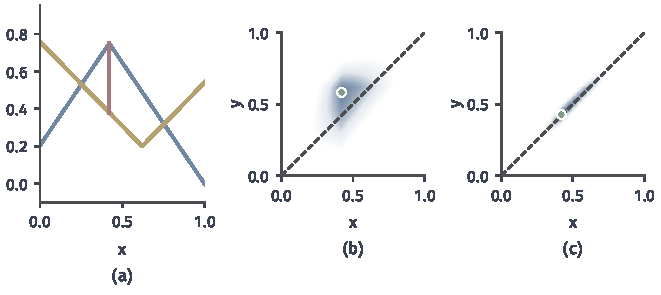
\includegraphics[width=112mm]{figures/06-differential-equations/02-partial-differential-equations/matplotlib/hj-doubling/figure.pdf}
  \caption{变量倍增。(a)$u$（蓝，凹折角）和$v$（黄，凸折角），红线段标出$u-v$的最大值。(b)、(c)$\Phi(x,y)$的正值，白色表示$\Phi\leq0$，蓝色越深值越大，绿点是极大点，虚线是对角线，$\delta=0.6$和$0.12$。}
  \label{fig:hj-doubling}
\end{BookInlineFigure}

\paragraph{初值问题}
下面是初值问题的比较原理。为了涵盖$H=p^2/2$这种关于$\bm{p}$不全局Lipschitz的情形，我们要求函数关于$\bm{x}$是Lipschitz的，这样只需要$H$在有界的$\bm{p}$上的性质。

\begin{theorem}[初值问题的比较原理]
\label{thm:hj-comparison}
设$H(t,\bm{x},\bm{p})$在$\lVert\bm{p}\rVert_2\leq R$的范围内关于全部自变量一致连续。设$u,v$在$\mathbb{R}^{d}\times[0,t_{\mathrm{f}}]$上有界、一致连续，关于$\bm{x}$是$R$-Lipschitz的，$u$是次解，$v$是上解。若$u(\cdot,0)\leq v(\cdot,0)$，则
\begin{equation}
  u\leq v\quad\text{在}\ \mathbb{R}^{d}\times[0,t_{\mathrm{f}}]\ \text{上}.
  \label{eq:hj-comparison}
\end{equation}
\end{theorem}

\begin{proof}
反设$\sigma=\sup(u-v)>0$。由连续性，存在$(\bar{\bm{x}},\bar{t})$，$\bar{t}<t_{\mathrm{f}}$，使$(u-v)(\bar{\bm{x}},\bar{t})>3\sigma/4$。对$\lambda,\delta>0$，记$\psi(t)=\lambda/(t_{\mathrm{f}}-t)$，并令
\[
  \begin{aligned}
    \Phi(\bm{x},\bm{y},t,s)={}&u(\bm{x},t)-v(\bm{y},s)-\psi(t)-\psi(s)\\
    &-\frac{\lVert\bm{x}-\bm{y}\rVert_2^2+(t-s)^2}{\delta^2}-\delta\bigl(\lVert\bm{x}\rVert_2^2+\lVert\bm{y}\rVert_2^2\bigr).
  \end{aligned}
\]
$\psi$在$t\to t_{\mathrm{f}}$时趋于无穷，二次项在无穷远处趋于负无穷，而$u,v$有界，所以$\Phi$在某点$(\bm{x}_0,\bm{y}_0,t_0,s_0)$取到最大值，且$t_0,s_0<t_{\mathrm{f}}$。先取$\lambda$充分小，此后只令$\delta\to0$，使得
\[
  \Phi(\bm{x}_0,\bm{y}_0,t_0,s_0)\geq\Phi(\bar{\bm{x}},\bar{\bm{x}},\bar{t},\bar{t})\geq\frac{\sigma}{2}.
\]

第一步估计最大点。记$C_0=\sup\lvert u\rvert+\sup\lvert v\rvert$。由上式，各惩罚项之和不超过$u(\bm{x}_0,t_0)-v(\bm{y}_0,s_0)\leq C_0$，所以
\[
  \begin{gathered}
    \lVert\bm{x}_0-\bm{y}_0\rVert_2\leq\sqrt{C_0}\,\delta,\qquad\lvert t_0-s_0\rvert\leq\sqrt{C_0}\,\delta,\\
    \delta\lVert\bm{x}_0\rVert_2\leq\sqrt{C_0\delta},\qquad\delta\lVert\bm{y}_0\rVert_2\leq\sqrt{C_0\delta}.
  \end{gathered}
\]

第二步说明$t_0,s_0>0$。若$t_0=0$，由$u(\cdot,0)\leq v(\cdot,0)$，
\[
  \frac{\sigma}{2}\leq u(\bm{x}_0,0)-v(\bm{y}_0,s_0)\leq v(\bm{x}_0,0)-v(\bm{y}_0,s_0).
\]
$s_0=\lvert t_0-s_0\rvert$，右端在$\delta\to0$时由$v$的一致连续性趋于零，矛盾。若$s_0=0$，同样用$u$的一致连续性得到矛盾。

第三步使用次解和上解的定义。记$\bm{p}=2(\bm{x}_0-\bm{y}_0)/\delta^2$。固定$(\bm{y}_0,s_0)$，函数$(\bm{x},t)\mapsto\Phi$是$u$减去$C^1$函数，它在$(\bm{x}_0,t_0)$取极大。测试函数的时间导数是$\psi'(t_0)+2(t_0-s_0)/\delta^2$，梯度是$\bm{p}+2\delta\bm{x}_0$，所以由次解条件，
\[
  \psi'(t_0)+\frac{2(t_0-s_0)}{\delta^2}+H\bigl(t_0,\bm{x}_0,\bm{p}+2\delta\bm{x}_0\bigr)\leq0.
\]

固定$(\bm{x}_0,t_0)$，$v$减去相应的$C^1$函数在$(\bm{y}_0,s_0)$取极小，测试函数的时间导数是$-\psi'(s_0)+2(t_0-s_0)/\delta^2$，梯度是$\bm{p}-2\delta\bm{y}_0$。由上解条件，
\[
  -\psi'(s_0)+\frac{2(t_0-s_0)}{\delta^2}+H\bigl(s_0,\bm{y}_0,\bm{p}-2\delta\bm{y}_0\bigr)\geq0.
\]

两式相减，$2(t_0-s_0)/\delta^2$抵消，得到
\[
  \psi'(t_0)+\psi'(s_0)\leq H\bigl(s_0,\bm{y}_0,\bm{p}-2\delta\bm{y}_0\bigr)-H\bigl(t_0,\bm{x}_0,\bm{p}+2\delta\bm{x}_0\bigr).
\]
由引理~\ref{lem:hj-lipschitz-touch}，两个梯度的长度都不超过$R$，所以可以用$H$的一致连续性。两组自变量的距离由第一步趋于零，右端趋于零。

而左端不小于$2\lambda/t_{\mathrm{f}}^2$，是一个与$\delta$无关的正数，矛盾。
\end{proof}

证明中每个假设的作用都能指出来。有界性让$\delta\lVert\bm{x}\rVert_2^2$这一项能把最大点留在有限范围内，这是增长条件的来源。一致连续性让第二步能把最大点推离$t=0$。Lipschitz条件和$H$的一致连续性负责最后一步。$\psi$的引入提供了严格的正数。

比较原理立刻给出唯一性和连续依赖。

\begin{theorem}[唯一性与数据稳定性]
\label{thm:hj-uniqueness}
在定理~\ref{thm:hj-comparison}的条件下，设$u$、$v$是黏性解，初值分别为$u_0$、$v_0$，$H$不依赖场值。则对$0\leq t\leq t_{\mathrm{f}}$，
\begin{equation}
  \sup_{\bm{x}}\lvert u(\bm{x},t)-v(\bm{x},t)\rvert\leq\sup_{\bm{x}}\lvert u_0(\bm{x})-v_0(\bm{x})\rvert.
  \label{eq:hj-stability}
\end{equation}
特别地，在这一函数类中，同一初值的黏性解至多一个。
\end{theorem}

\begin{proof}
记$K=\sup\lvert u_0-v_0\rvert$。$H$不依赖场值，所以$v+K$仍是黏性解，因为加常数不改变测试函数的导数。此时$u_0\leq v_0+K$，由比较原理得$u\leq v+K$。交换$u$、$v$得到另一半。$K=0$时就是唯一性。
\end{proof}

式~\eqref{eq:hj-stability}说明，解到解的映射在上确界范数下不扩张。图~\ref{fig:hj-order-preserved}用第~\ref{sec:hj-hopf-lax}节的公式算了一个例子：初值的差在$[0,0.6]$内，此后$u\leq v$一直保持，差的最大值始终不超过$0.6$，差的最小值保持为$0$。

\begin{BookInlineFigure}
  \centering
  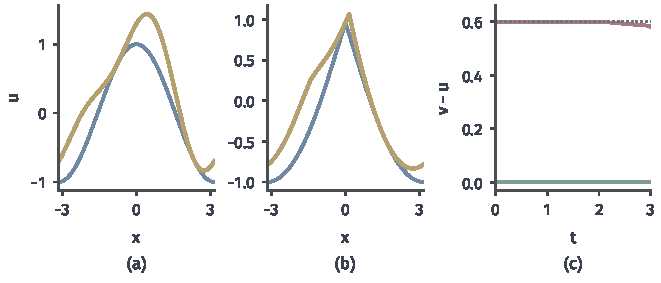
\includegraphics[width=112mm]{figures/06-differential-equations/02-partial-differential-equations/matplotlib/hj-order-preserved/figure.pdf}
  \caption{次序保持与上确界稳定性，$H=p^2/2$。(a)初值$u_0=\cos x$（蓝）和$v_0=\cos x+0.3+0.3\sin2x$（黄），$v_0\geq u_0$。(b)$t=1.2$的解，次序不变。(c)$v-u$的最大值（红）和最小值（绿）随时间的变化，虚线是初始最大差$0.6$。}
  \label{fig:hj-order-preserved}
\end{BookInlineFigure}

比较原理还给出简单的先验界。对$H=p^2/2$和例~\ref{ex:hj-cos}，常数$\pm1$都是经典解，$-1\leq\cos x\leq1$，所以在所有时刻$-1\leq u\leq1$。不解方程就知道了解的范围。

也可以用它解释凹槽为什么被排除。若$w$是上解，将它和次解$0$比较，初值都是$0$，比较原理给出$0\leq w$，而$w$在凹槽内为负。所以$w$不可能是上解，这就是例~\ref{ex:hj-notch-test}在底部折角处看到的失败。整体的比较结论，靠的正是接触点处的不等式。

条件不能随意去掉。取无界的初值$u_0=-x^2/2$，$H=p^2/2$，由特征线得到经典解
\[
  u(x,t)=-\frac{x^2}{2(1-t)},\qquad0\leq t<1.
\]
当$t\uparrow1$时，$u(x,t)\to-\infty$（$x\neq0$），没有办法延拓到$t\geq1$。有界性假设排除的就是这种从无穷远处传来的影响。

\paragraph{边值问题}
稳态的到达时间问题没有时间方向，上面证明中的$\psi$无从谈起，严格性要用别的办法得到。程函方程里可以把次解乘一个小于$1$的常数。

\begin{theorem}[程函方程的比较原理]
\label{thm:hj-comparison-eikonal}
设$\Omega\subset\mathbb{R}^{d}$有界开，$n\in C(\overline{\Omega})$，$n>0$。设$u,v\in C(\overline{\Omega})$分别是$\lVert\nabla u\rVert_2=n$在$\Omega$内的次解和上解，并且在$\partial\Omega$上$u\leq v$，则
\begin{equation}
  u\leq v\quad\text{在}\ \overline{\Omega}\ \text{上}.
  \label{eq:hj-comparison-eikonal}
\end{equation}
\end{theorem}

\begin{proof}
反设$\sigma=\max_{\overline{\Omega}}(u-v)>0$。取$\theta\in(0,1)$充分接近$1$，使$(1-\theta)\max\lvert u\rvert<\sigma/4$，于是$\sigma'=\max(\theta u-v)\geq3\sigma/4$，而在$\partial\Omega$上$\theta u-v\leq\sigma/4$。

对$\delta>0$，令
\[
  \Phi(\bm{x},\bm{y})=\theta u(\bm{x})-v(\bm{y})-\frac{\lVert\bm{x}-\bm{y}\rVert_2^2}{\delta^2},
\]
它在紧集$\overline{\Omega}\times\overline{\Omega}$上的最大点记为$(\bm{x}_\delta,\bm{y}_\delta)$。$\Phi$的最大值不小于$\sigma'$，所以惩罚项有界，$\lVert\bm{x}_\delta-\bm{y}_\delta\rVert_2\to0$。取子列使$\bm{x}_\delta,\bm{y}_\delta\to\bm{z}$，由连续性
\[
  \theta u(\bm{z})-v(\bm{z})\geq\sigma'\geq\frac{3\sigma}{4}.
\]
这说明$\bm{z}\notin\partial\Omega$，$\delta$小时$\bm{x}_\delta,\bm{y}_\delta$都在$\Omega$内。

记$\bm{p}=2(\bm{x}_\delta-\bm{y}_\delta)/\delta^2$。固定$\bm{y}_\delta$，$u$减去光滑函数在$\bm{x}_\delta$取极大，测试函数的梯度是$\bm{p}/\theta$，由次解条件$\lVert\bm{p}\rVert_2/\theta\leq n(\bm{x}_\delta)$。固定$\bm{x}_\delta$，由上解条件$\lVert\bm{p}\rVert_2\geq n(\bm{y}_\delta)$。两式合并，得到
\[
  n(\bm{y}_\delta)\leq\theta\,n(\bm{x}_\delta).
\]
令$\delta\to0$，$n(\bm{z})\leq\theta n(\bm{z})$，与$n(\bm{z})>0$、$\theta<1$矛盾。
\end{proof}

取$n=1/c$，$c$连续且有正的上下界，这个定理就适用于第~\ref{sec:hj-problem}节的到达时间问题，方程写成$c\lVert\nabla T\rVert_2-1=0$和$\lVert\nabla T\rVert_2-n=0$时次解、上解的条件相同，因为$c>0$不改变不等号方向。定理~\ref{thm:hj-distance}的距离函数在有界区域上是边值为零的唯一黏性解。

正性$n>0$的作用是提供严格性。若$n$在某点为零，可以看到比较原理失败。在$(-1,1)$上取$\lvert u'\rvert=2\lvert x\rvert$，$u(\pm1)=0$，这里$n(0)=0$，相当于速度在原点为无穷大。则
\[
  u=1-x^2\qquad\text{和}\qquad u=x^2-1
\]
都是$C^1$的经典解，因而都是黏性解，见图~\ref{fig:hj-boundary-failures}(a)。这就破坏了唯一性。

\begin{BookInlineFigure}
  \centering
  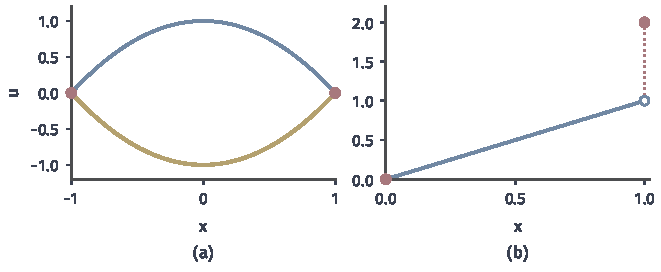
\includegraphics[width=112mm]{figures/06-differential-equations/02-partial-differential-equations/matplotlib/hj-boundary-failures/figure.pdf}
  \caption{边值问题的两种失败。(a)$\lvert u'\rvert=2\lvert x\rvert$，$u(\pm1)=0$（红点）有两个经典解$1-x^2$（蓝）和$x^2-1$（黄）。(b)$\lvert u'\rvert=1$，$u(0)=0$，$u(1)=2$（红点）：连续解取$u=x$，在右端得到$u(1)=1$（空心点），边值$2$没有被达到。}
  \label{fig:hj-boundary-failures}
\end{BookInlineFigure}

边界数据不相容时，问题出在另一处。在$(0,1)$上取$\lvert u'\rvert=1$，$u(0)=0$，$u(1)=2$。方程要求$u$是$1$-Lipschitz的，$u(1)$不可能等于$2$。自然的候选是
\[
  u(x)=\min\{0+x,\ 2+(1-x)\}=x,
\]
它在$(0,1)$内是黏性解，但在右端取值$1$，边值$2$被丢掉了，见图~\ref{fig:hj-boundary-failures}(b)。这对应第~\ref{sec:hj-problem}节的相容性条件。边值问题的比较原理假定函数已经在边界上按要求比较，它并不保证任何数据都能取到。

初值问题不会出现边值丢失，这里的差别列在表~\ref{tab:hj-comparison-cases}中，一种情形的结论不能搬到另一种情形。

\begin{BookInlineTable}
  \centering
  \begin{tabular}{lll}
    \toprule
    & 初值问题 & 程函边值问题\\
    \midrule
    严格性来源 & 时间函数$\psi$ & 系数$\theta<1$与$n>0$\\
    比较的部位 & $t=0$，全空间 & 边界$\partial\Omega$\\
    无穷远的控制 & 有界性、$\delta\lVert\bm{x}\rVert_2^2$ & 有界区域\\
    数据的限制 & 有界且Lipschitz & 需要相容，否则边值丢失\\
    条件破坏时 & 爆破、非唯一 & $n$有零点时非唯一\\
    \bottomrule
  \end{tabular}
  \caption{初值问题与边值问题的比较原理。}
  \label{tab:hj-comparison-cases}
\end{BookInlineTable}
